{
  \newcommand{\colorgradientbox}{%
    \tikz[baseline=-0.5ex]{
      \node[minimum height=1em, minimum width=3em, draw=black, line width=0.8pt,
            shading=horizontal, left color=white, right color=red] (char) {};
    }\;%
  }

  \newcommand{\solidcolorbox}{%
    \tikz[baseline=-0.5ex]{
      \node[minimum height=1.0em, minimum width=1.0em, draw=black, line width=0.8pt, fill=green!20!white] (char) {};
    }\;%
  }

  \begin{figure}[htbp]
    \centering    
    \begin{subfigure}{.33\textwidth}
        \centering
        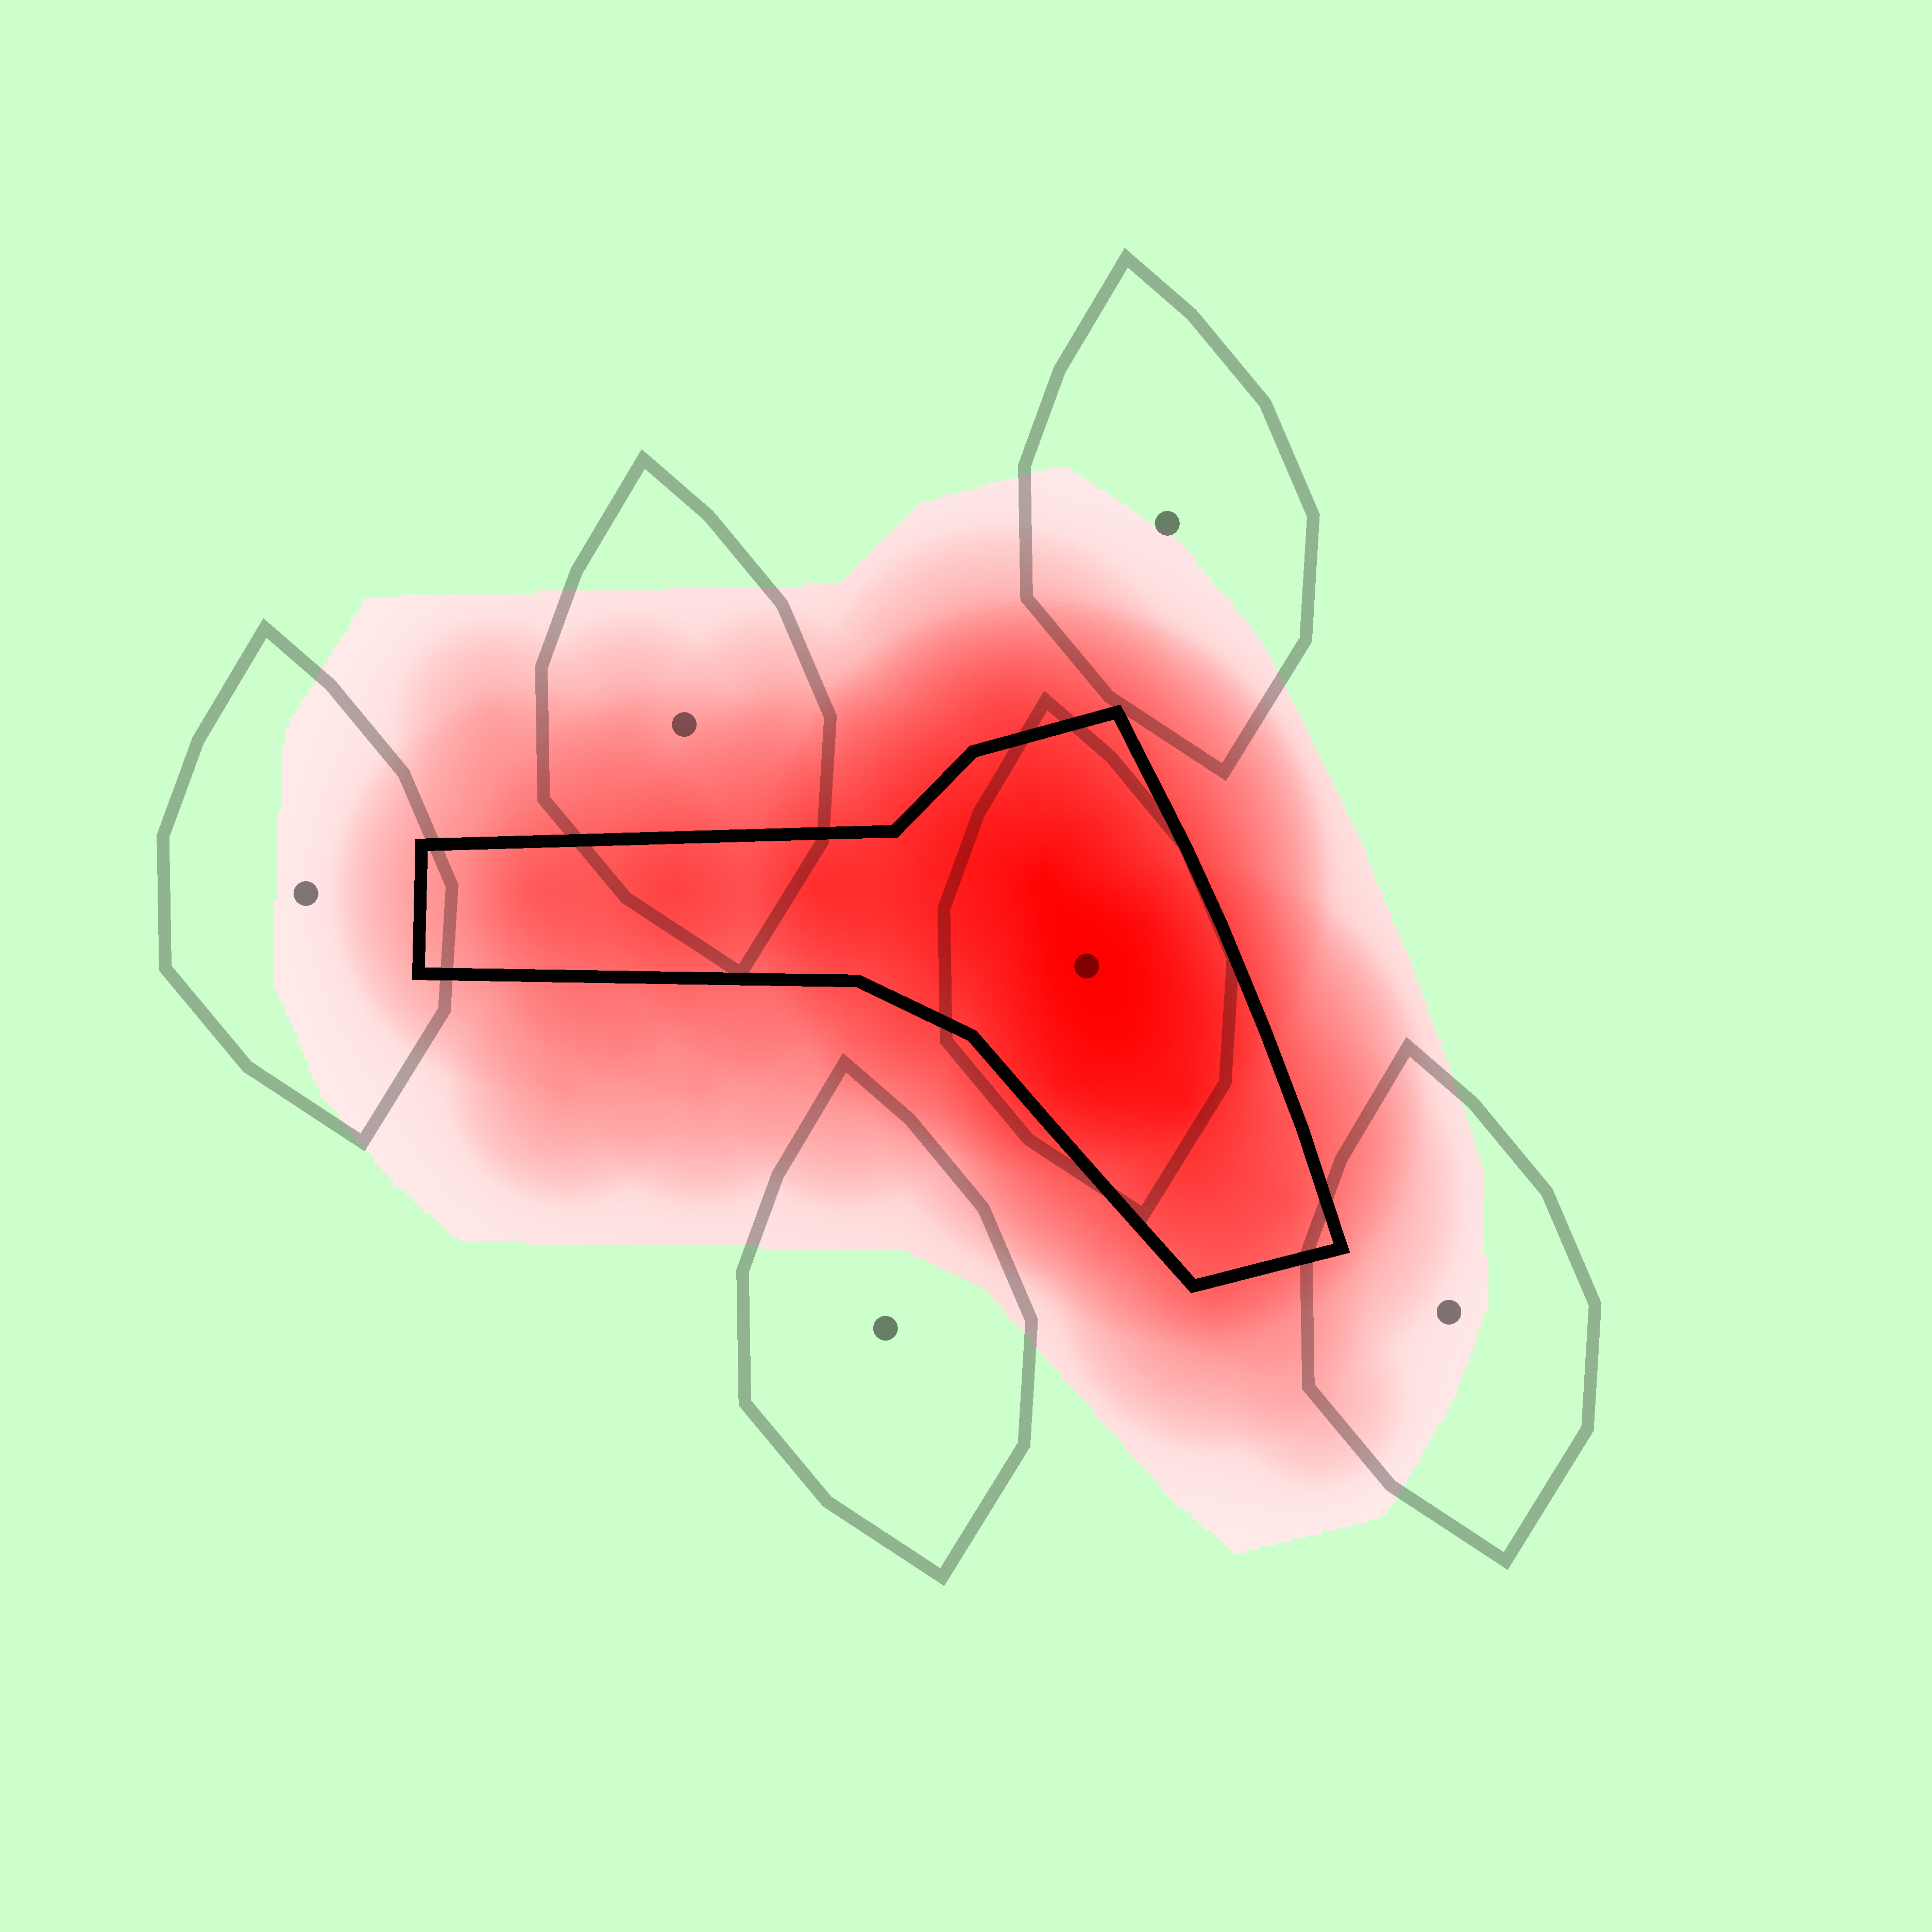
\includegraphics[trim={60 100 220 180}, clip=true, width=1.0\textwidth]{overlap_decay.svg.pdf}
        \caption{2D}
    \end{subfigure}
    \hspace{0.1\textwidth}
    \begin{subfigure}{.33\textwidth}
        \centering
        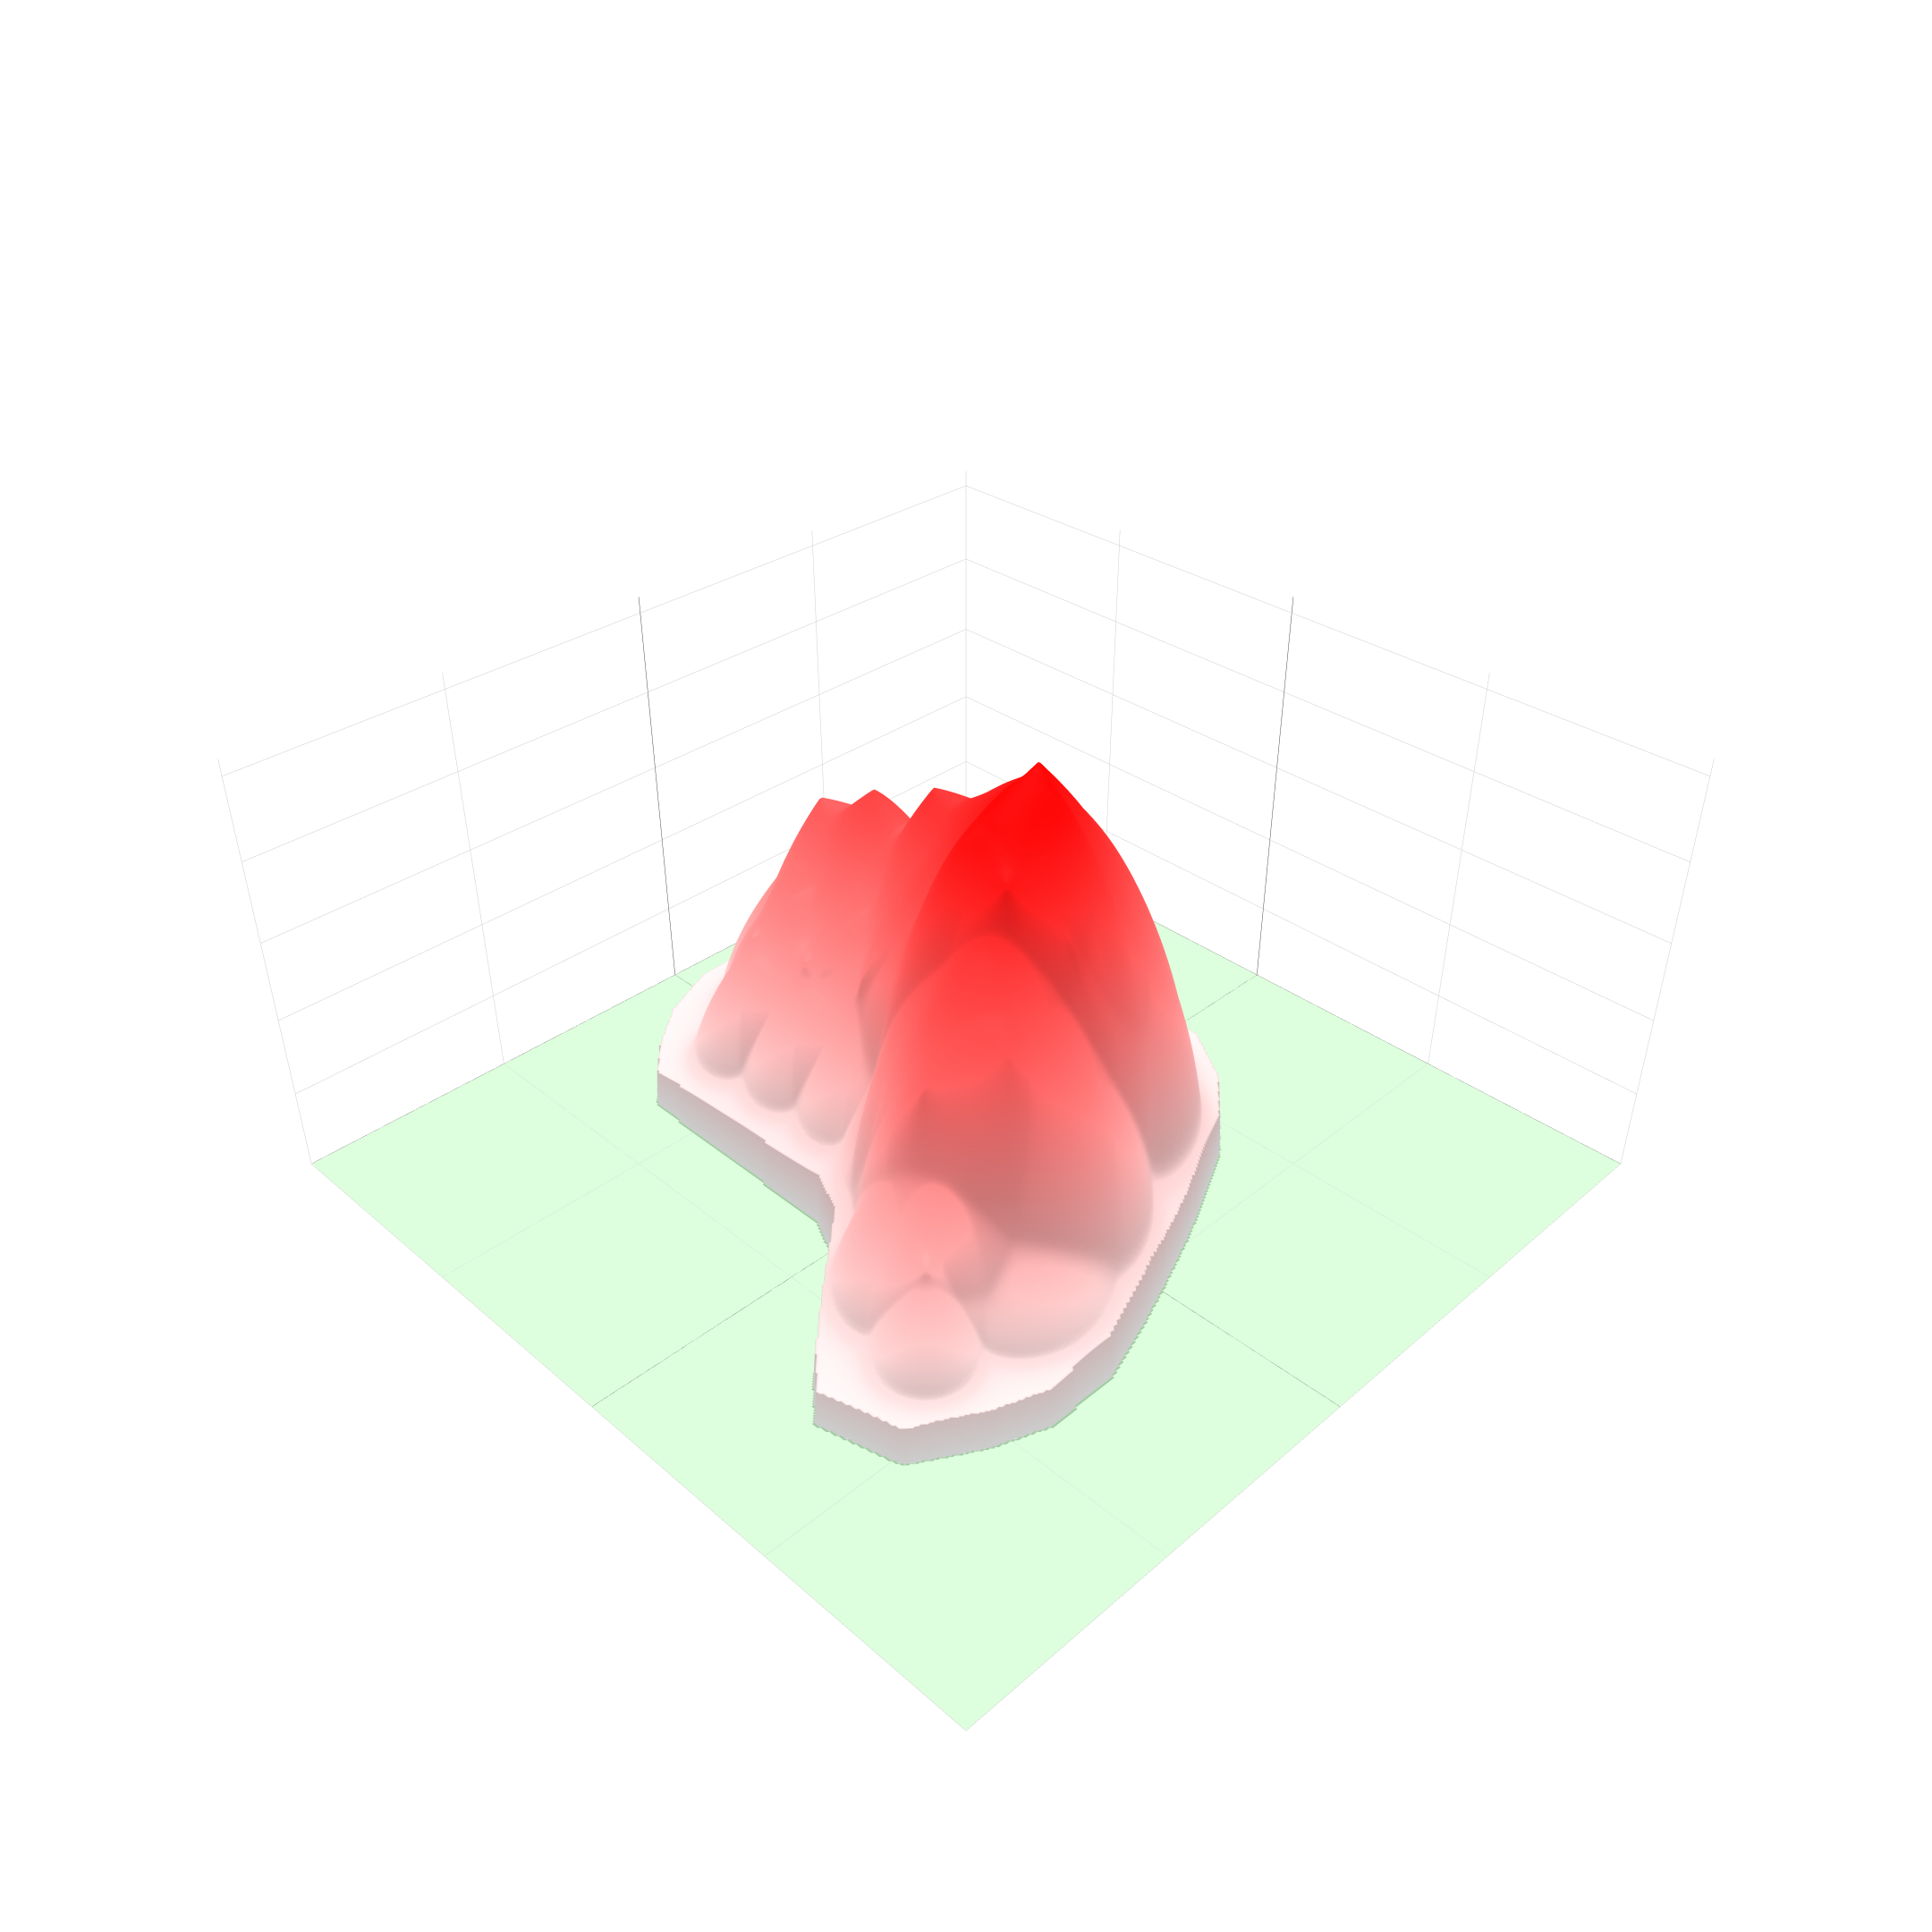
\includegraphics[trim={600 400 600 800}, clip=true, width=1.0\textwidth]{overlap_3d_decay.png}
        \caption{3D}
    \end{subfigure}
    \caption{Visualization of the decaying overlap proxy for the same pair of items from Figure~\ref{fig:poles}.
    {\protect\solidcolorbox}: feasible, {\protect\colorgradientbox}: \nameref{alg:overlap_area_proxy_decay}.}
    \label{fig:overlap_decay}
  \end{figure}
}